\documentclass[12pt,a4paper,openany]{book}
\usepackage{graphicx}
\usepackage{geometry}
\usepackage{fancyhdr}
\usepackage[style=verbose]{biblatex}
\usepackage{subfiles}
\usepackage{makecell}
\usepackage{fancyhdr}
\usepackage{titlesec}
\usepackage{lipsum}

%Header for the first page
\pagestyle{fancy}
\fancyhf{}
\setlength{\headheight}{45pt}

\lhead{
  
\includegraphics[width=3cm]{img/htlwrn_logo}  
}
\chead{\Large HTBLuVA Wiener Neustadt \\ \normalsize Höhere Lehranstalt für Informatik}
\rhead{
  
\includegraphics[width=3cm]{img/htlwrn_logo2}
}

\newcommand{\parseauthor}[3]{\makecell{#1 \\ #2} & #3}

%definitions for easier costumization
\def \title {DIPLOMARBEIT}
\def \subtitle {Localisation via ML Methods}
\def \year {2019/20}
\def \authors { \parseauthor{Rolle x}{Ida Hönigmann}{5AHIF}\\
                \parseauthor{Rolle y}{Peter Kain}{5AHIF}}
\def \supervisor {MMag. Dr. Michael Stifter}
\def \declauthors{ Ida HÖNIGMANN & Peter KAIN}

\graphicspath{ {img/} }

\setlength{\parindent}{0em}

\geometry{
 a4paper,
 left=30mm,
 top=50mm,
 }

\addbibresource{main.bib}


\begin{document}
	%include titlepage
	
\begin{titlepage}
  \thispagestyle{fancy}
  \begin{center}
    \Huge
    \texttt{\textbf{\title}} \\
    \vspace{1cm}
    \LARGE
    \bf{\subtitle}\\
  \end{center}
  \vspace{2cm}
  \begin{flushleft}
    \normalsize
    \textbf{Ausgeführt im Schuljahr \year \space von:}\\
    \vspace{2mm}
     \begin{tabular}{p{.5\textwidth}l}
        \authors
      \end{tabular} \\
  \end{flushleft}
  \vfill
  \begin{center}
      \vspace{1cm}
      \textbf{Betreuer / Betreuerin:}\\
    \vspace{2mm}
    \begin{tabular}{l}
      \supervisor
    \end{tabular}
    
    \vspace{2cm}
    
    Wiener Neustadt, am \today
    
    \rule{14cm}{0.4mm}
    
    \begin{tabular}{p{.4\textwidth}p{.4\textwidth}}
      \scriptsize{Abgabevermerk:} & \scriptsize{Übernommen von:}
    \end{tabular}
    
  \end{center}
\end{titlepage}

	
	%include acknowledgements, abstract and documentation
	
	\pagestyle{plain}
	
	\frontmatter
	
	\pagenumbering{roman}
	% english word for 'eidestattliche erklärung?'

\addcontentsline{toc}{section}{Eidestattliche Erklärung}
\section*{Eidestattliche Erklärung}

\vspace{10mm}

\normalsize
Hiermit erkläre ich an Eides statt, dass ich die vorliegende Arbeit selbstständig und ohne fremde Hilfe verfasst und keine anderen als die im Literaturverzeichnis angegeben Quellen und Hilfsmittel verwendet habe. Insbesondere versichere ich, dass ich alle wörtlichen und sinngemäßen Übernahmen aus anderen Werken als solche kenntlich gemacht habe.

\vspace{1cm}

Wiener Neustadt am \today \\

\vspace{1cm}

{\bf Verfasser / Verfasserinnen:} \\

\vspace{2cm}

  \begin{tabular}{p{.4\textwidth}p{.4\textwidth}}
    \declauthors
  \end{tabular}

	\tableofcontents
	\newpage
	\chapter{Acknowledgement}

The authors would like to thank ...
	\addcontentsline{toc}{section}{Kurzzusammenfassung}
\section*{Kurzzusammenfassung}

\vspace{10mm}

\normalsize
TODO

\newpage

\addcontentsline{toc}{section}{Abstract}
\section*{Abstract}

\vspace{10mm}

\normalsize
TODO

\end{document}

	
	%include thesis
	
	\mainmatter
	\pagenumbering{arabic}
	\chapter{Introduction}

\textbf{Author: Ida Hönigmann}

\vspace{2mm}

Robots are getting more and more mobile. While a few years ago their usage was mostly limited to aid factory automation, robots have found widespread adoption in a multitude of industries, such as self driving cars and autonomous delivery drones.
A challenge frequently encountered is navigating in unknown environments, which either requires the robot to sense specific characteristics of its surroundings or to communicate with some external system.

The problem of navigation has been looked at from many different angles. One popular approach in mobile robotics is to use the GPS, an external positioning system. In order to determine the position of a robot using the GPS, it has to establish communication with at least four satellites. The exact position of each satellite as well as the current time is broadcast by the satellites. By measuring the time needed for the signal to reach the robot, the position can be calculated up to three meters accurately.

However, in some cases positioning a robot using external positioning methods is not possible. In the case of the GPS this can be due to obstacles interfering with the radio signals send by the satellites, for example occurring inside a building.
In comparison, we focus on a system that can navigate in outdoor as well as in indoor environments. 

\section{Goal}
The goal of this diploma thesis is to implement a system which can localize a robot using no other sensors than a camera. This limitation was purposely chosen as our system will be used by future robotic students at our school and many robot systems used in the field of education are only poorly equipped with sensors that are able to detect its environment. One sensor used in the field of educational robotics is the either already equipped, or easily mountable camera.

As part of our work we not only want to implement an easy to use API for future robotic students, but to also show the possibilities and advantages of machine learning in localisation.

In order to accomplish precise localisation in various different surroundings, we plan on implementing a neural network. The neural network should take images, taken by the camera, as an input, and outputs the relative distance to any object shown in the images. By using machine learning we hope to be less dependent on a specific situation or setup in comparison to different camera based localisation methods. For example the localisation should work on objects varying in size and shape, as well as in different situations of lighting.

\section{Motivation}
In July 2019 the two authors of this work participated in the aerial tournament at the Global Conference on Educational Robotics held in Norman, Oklahoma. One of the two main challenges encountered at this tournament was landing a drone next to some randomly placed object, which colour, shape and size was known in advance.

The second challenge we faced was flying from one side of randomly placed cardboard boxes to the other. The cardboard boxes, representing a mountain, are placed in one of various configurations, one of which can be seen in figure~\ref{pic:introduction_motivation_mountain}.

\begin{figure}[h]
	\centering
	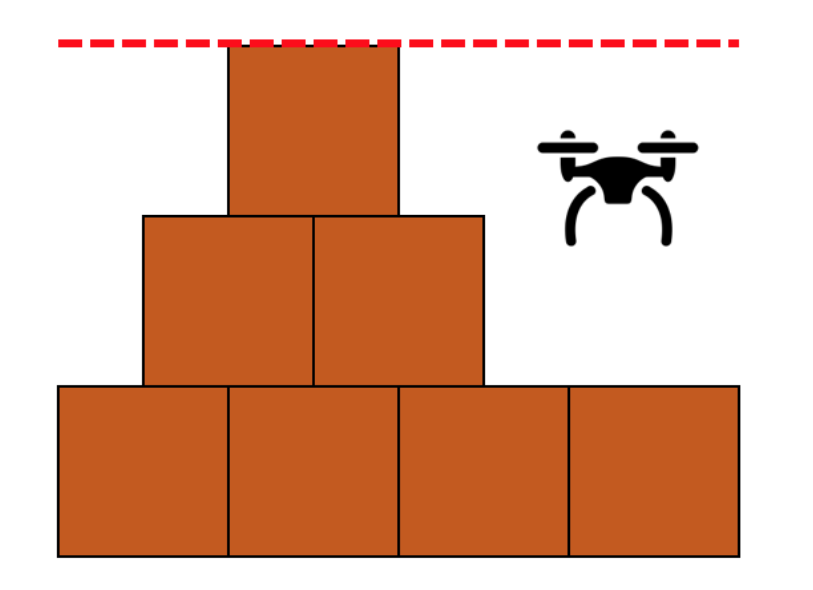
\includegraphics[width=2.5in]{img/introduction_motivation_mountain.png}
	\caption{Seven cardboard boxes, representing a mountain, are placed in a random configuration. The team scores points if the drone passes the mountain while staying under the height limit indicated by the red dotted line.}
	\label{pic:introduction_motivation_mountain}
\end{figure}

The drones used at this aerial tournament are equipped with a camera, while lacking any other sensor that can be used to detect the obstacles and game items. Therefore we needed to be able to detect the distance to the object and the cardboard boxes using only the camera. At the Global Conference on Educational Robotics we decided to detected the object based on its colour, but had to invest quite some time to tweak the values to get the localisation working correctly. Therefore we want to research and implement a method that is more robust than the colour based one.

\filbreak

	\chapter{Project Management}

\textbf{Author: } 

\section{Section}
\textbf{[TODO]}
\newline
\lipsum[1]

\section{Kanban}
:-)

\filbreak
	\chapter{Study of Literature}

\textbf{Author: } 

\section{Different Approaches to the Problem}

\section{Depth perception}
[TODO: humans, two eyes - gleich wie bei unserem Aufbau]

\subsection{Depth sensation}
[TODO: Pigeons, deer, children (visual cliff)]

\section{Stereo Camera}
The challenge of sensing distances to various objects has been solved using stereo vision cameras. Computer stereo vision systems use two horizontally displaced cameras to take two images which then are both processed together to gather the information on the depth of the images. This process can be rather complicated as the distortions (more specifically the barrel distortion and the tangential distortion) of the images have to be undone, before the two images are projected onto a common plane, a disparity map can be created by comparison of the two images and a 3d point cloud can be generated from it. In most robotics applications this point cloud is then filtered in search of some object, which distance was sought-after.

\subsection{Distortion}
Barrel distortion occurs when the lens used by the camera has a higher magnification at the centre of the image than at the sides. This distortion can be visualized as seen in Figure~\ref{pic:methodology_stereoCamera_distortion_barrelDistortion}.

\begin{figure}[h!]
	\centering
	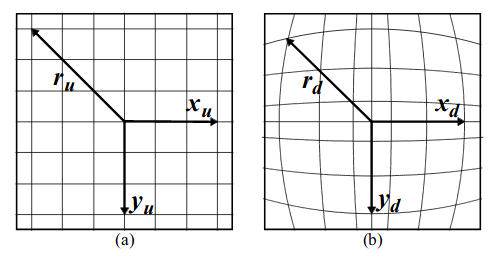
\includegraphics[width=4.5in]{img/methodology_stereoCamera_distortion_barrelDistortion.png}
	\caption{The left shows the original image composed of straight horizontal and vertical lines. On the right image the effect of the barrel distortion can be perceived, which causes the lines to curve toward the outside of the image, causing the lines to appear in a barrel like shape.[TODO: change image to own]}
	\label{pic:methodology_stereoCamera_distortion_barrelDistortion}
\end{figure}

To undo this distortion the pixel values in an undistorted image have to be calculated based on the pixel values in the distorted image.

\begin{equation}
r_u = r_d(1+k r_d^2)
\end{equation}

describes the calculation which computes the distance from the centre in the undistorted image ($r_u$) based on the distance from the centre in the distorted image ($r_d$) and some distortion parameter $k$, which is specific to the lens used. Gribbon et.al. note in their work \footcite{Gribbon_Barrel_Distortion_Correction_Algorithm} that this rarely is an integer value, therefore different equations are proposed:

\begin{equation}
x_d = x_u M(k,r_u^2) \hspace{30pt} y_d = y_u M(k, r_u^2)
\end{equation}

where the magnification factor $M(k,r_u^2)$ is

\begin{equation}
M(k,r_u^2) = \frac{1}{1+k * M(k,r_u^2)^2 * r_u^2}
\end{equation}

Tangential distortion in comparison to barrel distortion displaces points along the tangent of a circle placed at the centre of the image as seen in Figure~\ref{pic:methodology_stereoCamera_distortion_tangentialDistortion}.

\begin{figure}[h!]
	\centering
	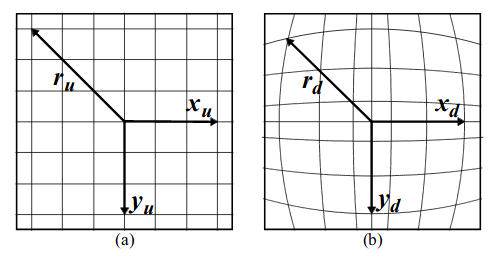
\includegraphics[width=2in]{img/methodology_stereoCamera_distortion_tangentialDistortion.png}
	\caption{A point $P$ is distorted along the tangent $t$ of a circle placed at the middle of the image $C$ with a radius $r$ to a point $P'$. Distortions of this form are called tangential distortions.}
	\label{pic:methodology_stereoCamera_distortion_tangentialDistortion}
\end{figure}

The radius of the circle in Figure~\ref{pic:methodology_stereoCamera_distortion_tangentialDistortion} is dependent on the point $P$. It can be calculated as the length between $P$ and $C$. The length of the vector $PP'$ is not uniform for all points and therefore depends on point $P$.

\subsection{Image Rectification}
Image Rectification projects multiple images taken from different points of view onto a common plane. 

\begin{figure}[h!]
	\centering
	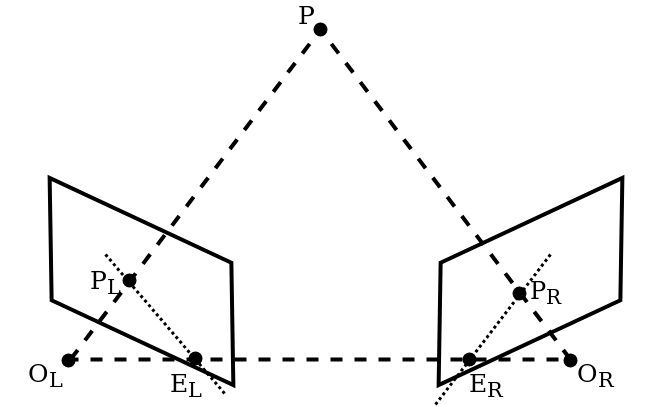
\includegraphics[width=4in]{img/methodology_stereoCamera_imageRectification.png}
	\caption{Two images containing some point $P$ are taken from the two points $O_L$ and $O_R$. Point $P$ is projected in the image planes as points $P_L$ and $P_R$. $E_L$ and $E_R$ depict the epipoles.}
	\label{pic:methodology_stereoCamera_imageRectification}
\end{figure}

Chan et. al. propose an image rectification algorithm \footcite{Chen_New_Image_Rectification_Algorithm}, which follows this sequence of events:

\begin{enumerate}
	\item At least seven matching points visible on both images are found.
	\item The fundamental matrix (as well as the epipoles) are estimated.
	\item The common region is identified (using epipolar geometry constraints).
	\item The epipolar line is transferred and the Bresenham algorithm\footcite{Bresenham_Linear_Algorithm_For_Incremental_Digital_Display_Of_Circular_Arcs} is used to extract pixel values.
	\item The rectified image is resampled.
\end{enumerate}

\subsection{Disparity Map}

\subsection{3d point cloud}


[Input: Paper (gleiches Problem ohne NN) finden - Peter]

[Input: Video (eine Kamera, Entfernung zu Punkt (größe bekannt)) finden (ohne NN) - Peter]


[Vielleicht ist irgendetwas davon spannend:
Links im Tex file
%https://ieeexplore.ieee.org/abstract/document/6399589
%https://ieeexplore.ieee.org/abstract/document/100062
%https://ieeexplore.ieee.org/abstract/document/6079296
%https://www.sciencedirect.com/science/article/pii/S0957417414008161
%http://neuralnetworksanddeeplearning.com/chap1.html
%https://patents.google.com/patent/US8164628B2/en
%https://apps.dtic.mil/docs/citations/ADA366182
%https://ieeexplore.ieee.org/abstract/document/1087003
%https://digital-library.theiet.org/content/conferences/10.1049/cp.2010.0495
%https://www.isca-speech.org/archive/interspeech_2010/i10_1045.html
%https://ieeexplore.ieee.org/abstract/document/6639344
%https://www.sciencedirect.com/science/article/pii/B9780127412528500108
%https://en.wikipedia.org/wiki/Visual_cliff#The_study_in_different_species
%https://science.sciencemag.org/content/145/3634/835
%https://en.wikipedia.org/wiki/Visual_cliff
%https://en.wikipedia.org/wiki/Depth_perception
]

\section{LIDAR}

\section{Structure from Motion}

\section{Feature Tracking}


\filbreak
	\chapter{Methodology}

\textbf{Author: } 

\section{Challenges in the use of Stereo Cameras}
Since many drones used in educational robotics can only carry a limited amount of weight it is not possible to attach a stereo camera to such a robot. Instead the functionality of a stereo camera on such a drone system can be mimicked by taking the first image, flying to a second position, located horizontally next to the first one and taking the second image. This process in not as precise as a stereo camera, where the two lenses are always positioned at an exact interval from one another. Therefore the output of this system might not work as reliable. Additionally other factors, such as differences in the two images due to some time passing between the taking of the images can have an effect on the accuracy.

Therefore the authors try to approach this challenge from the machine learning point of view. Neural networks can be taught to work with different changes in the environment and still return results with a superior quality to conventional implementation.

\section{Generating data}
Neural Networks require huge amounts of data to work reliably. Because of the author's limited time frame this test data will be generated with the help of Blender 2.8. Blender is a free program for designing and animating 3D objects, which also supports scripting with python to add or remove objects from a scene. The authors will use this capability to generate the huge amounts of test data needed from the perspectives of the 2 cameras, which point to a specific object in the scene. This enables the authors to use and train a neural network, since shooting the amount of pictures needed by hand would take too long to consider this idea.

\subsection{Blender}
Besides 3D-modelling Blender enables the user to perform various different actions, such as laying out scenes, UV-Editing, shading, animating and rendering. Additionally scenes can be modified by executing Python scripts. Figure~\ref{pic:methodology_generatingData_blender_startscreen} shows the interface of Blender 2.8 with the default file loaded.

\begin{figure}[h!]
	\centering
	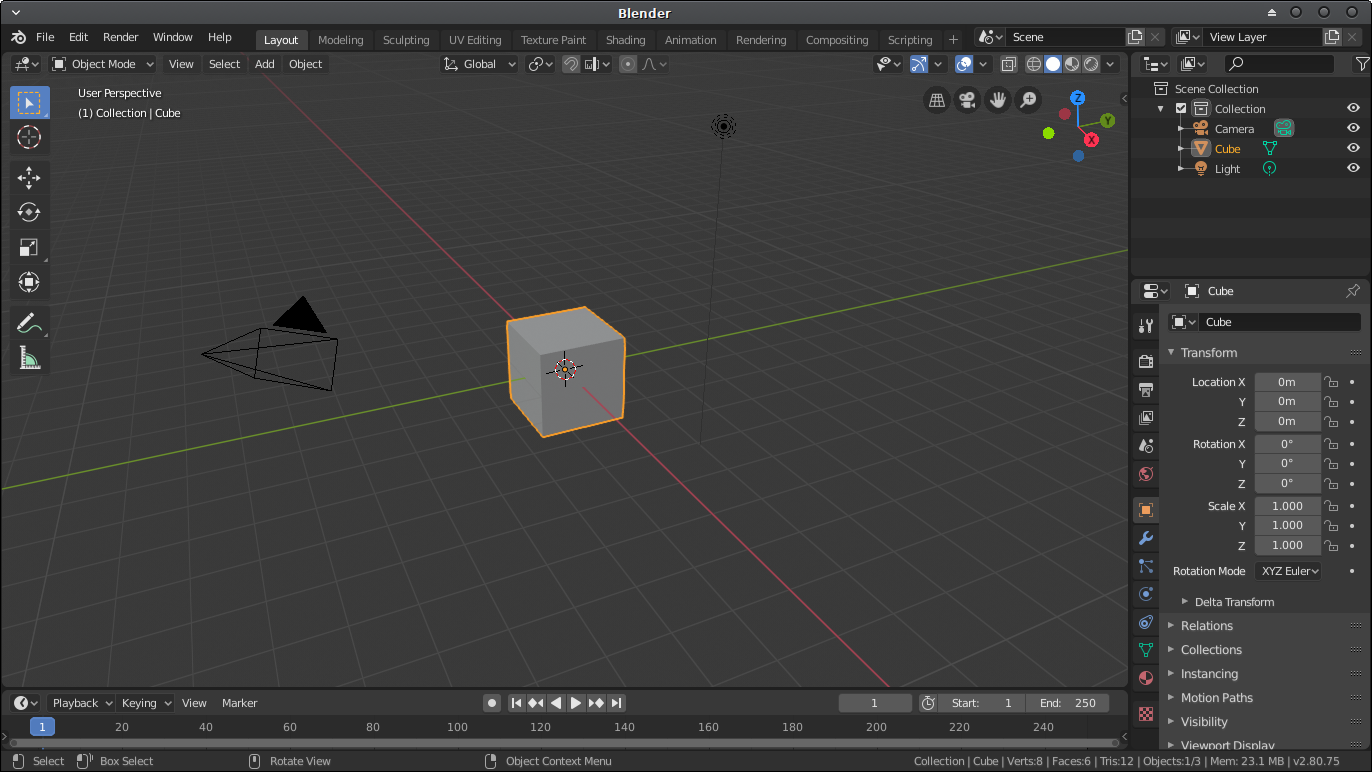
\includegraphics[width=6.5in]{img/methodology_generatingData_blender_startscreen.png}
	\caption{Blender interface after startup. The default scene features a grey cube, a camera (left of the cube) and a light source (black dot and circle positioned on the top right of the cube).}
	\label{pic:methodology_generatingData_blender_startscreen}
\end{figure}

The authors decided to extensively use the scripting function in their work. One example of a Python script, that can be executed in blender is the following code:

\begin{lstlisting}[language=python]
import bpy

# Selects all cubes and deletes them
bpy.ops.object.select_all(action='DESELECT')
bpy.ops.object.select_by_type(type='MESH')
bpy.ops.object.delete()

# Adds a new cube
bpy.ops.mesh.primitive_cube_add(size=3, enter_editmode=False, location=(4, 2, 0))

# Adds a new material representing the colour red
bpy.ops.material.new()
material = bpy.data.materials[-1]
material.name = 'Red'
material.diffuse_color = (0.8, 0.1, 0.1, 1)

# Apply material onto the newly created cube object
bpy.context.active_object.data.materials.append(material)
\end{lstlisting}

This code first clears the scene from other meshes (because running the script twice would place the new cube inside the old cube). Then it adds a new mesh in form of a cube at the given location. Next we want to add some color to the cube. For this to work a material is needed, which is basically a specification of how the surface of the object will look like. Advanced materials can represent raw or reflective surfaces, but in order to keep it simple this material will just represent a red surface (represented in red/green/blue/alpha channels ranging from 0.0 (for 0) to 1.0 (for 255)). Lastly the created material is applied to the object. The final result can be seen below:

[TODO: Add image]

Using similar Python scripts the authors will generate the image data necessary as well as perform the calculation of the distance which will be specified as the correct values to train the neural network on.

\section{Image preprocessing}
After the test images have been rendered with the help of Blender some image preprocessing is required. For example the machine learning component of this project should take two images as an input. To simplify the input the two images will simply be placed next to each other to form a new image twice as wide as the original images. This process is visualized in Figure~\ref{pic:methodology_imagePreprocessing_imageMerge}. Other preprocessing measures that have to be taken are downscaling the image, as to not have too many weights in the first layer of the neural network.

\begin{figure}[h!]
	\centering
	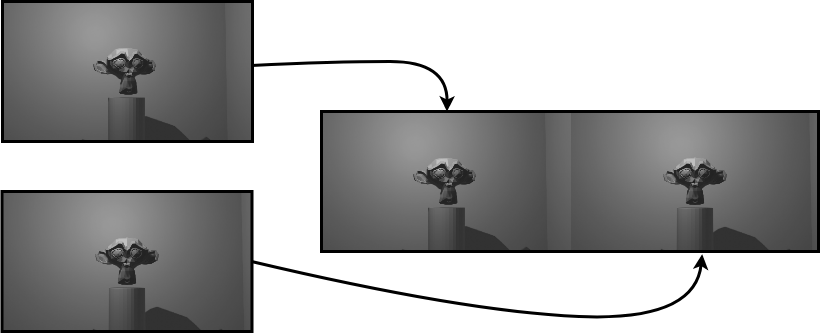
\includegraphics[width=6.5in]{img/methodology_imagePreprocessing_imageMerge.png}
	\caption{Two greyscale renders showing the same object from two different camera positions in Blender are merged into one picture which can be feed into the neural network component.}
	\label{pic:methodology_imagePreprocessing_imageMerge}
\end{figure}

Additionally, the authors decided to experiment if manipulating these test images further would result in differences of distance perception by the neural network or if they would speed up or slow down the learning phase. These manipulations are done using OpenCV and Python3. OpenCV provides many image manipulation tools. For this project the authors chose the following methods of image manipulation:

\begin{table}[h!]
	\begin{tabular}{|l|l|}
		\hline
		\bfseries Name & \bfseries Description \\
		\hline
		Greyscale & A greyscale image is an image with only one value for the red, green and \\
		& blue colour channels, resulting in different shades of grey instead of usual \\
		& colours. \\
		\hline
		Resolution & Resolution refers to the number of pixels placed in each dimension \\
		& (width and height). \\
		\hline
		Cropping & When cropping an image an unwanted part located at the peripheral areas \\
		& of the image is removed. \\
		\hline
		Saturated & Saturated images feature stronger colours, which makes them easier to \\
		& distinguish from another. \\
		\hline
		Brightness & Brightening images can make colours harder to distinguish from another. \\
		& Additionally it can lead to the same problems encountered in overexposed \\
		& images, such as part of the image being completely white and therefore not \\
		& providing any information. \\
		\hline
	\end{tabular}
\end{table}

\section{Neural Network}
The authors decided to use a software framework called TensorFlow for the first implementation of the neural network. This has the following two advantages: using Tensorflow allows for a low effort proof of concept and it makes testing out different configurations (e.g. number of hidden layers or filters in image preprocessing) of the neural network easier.

After it has been shown that the challenge of detecting the distance to an object can be solved using machine learning, the authors plan on implementing a neural network in C++ on their own. The knowledge gained in the TensorFlow implementation will be used in the C++ implementation, which hopefully will make the work less time consuming.

\section{TensorFlow}
As machine learning has gained popularity in recent years the demand for applicable frameworks grew. One of the most popular is called TensorFlow. It was developed by Google for internal use and was published under the Apache License 2.0 on the \nth{9} of November 2015.

TensorFlow supports APIs for Python, C, C++, Go, Java, JavaScript and Swift.
Due to its popularity third party APIs for C\#, R, Scala, Rust and many more were developed.

Its use cases reach from categorizing handwritten digits to YouTube video recommendations, one of the many applications Google use it for.

Tom Hope et al. describe TensorFlow as a software framework for numerical computations based on dataflow graphs \footcite[page 6]{Hope_Learning_TensorFlow}.

\subsection{Computation graph}
To compute a value using TensorFlow a computation graph has to be constructed. In this graph each node corresponds to an operation, such as subtraction or division. By connecting these nodes via edges the output of one node can be fed as input into another node. One example of such a computation graph can be seen in Figure~\ref{pic:methodology_tensorflow_computationGraph}.

\begin{figure}[h!]
	\centering
	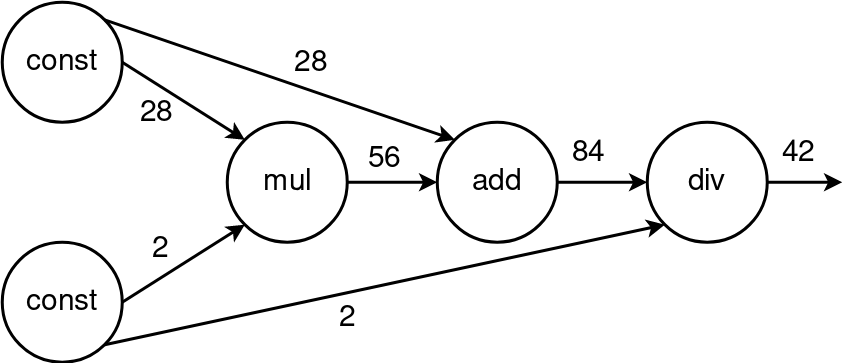
\includegraphics[width=4.5in]{img/methodology_tensorflow_computationGraph.png}
	\caption{Each node represents an operation, where $const$ stands for a constant value, $add$ for addition, $mul$ for multiplication and $div$ for division. Edges, represented by arrows, connect nodes. The information shared between the nodes is described by the numbers written next to the edges. This computational graph calculates the result of the arithmetic expression $(28 * 2) + 28 / 2$.}
	\label{pic:methodology_tensorflow_computationGraph}
\end{figure}

The implementation of the computation graph, shown in Figure~\ref{pic:methodology_tensorflow_computationGraph}, in Python could look as follows:

\begin{lstlisting}[language=python]
import tensorflow as tf

a = tf.constant(28)
b = tf.constant(2)

c = tf.multiply(a, b)
d = tf.add(a, c)
e = tf.divide(d, b)

with tf.Session() as sess:
out = sess.run(e)

print(out)
\end{lstlisting}

The first line specifies that the TensorFlow functionality should be imported. Line 3 and 4 define the two constant values and assigns them the values 28 and 2 respectively. In line 6 to 8 the other nodes of the graph are specified. E.g. in line 6 a new node, named $c$, is created and the output of node $a$ and node $b$ are connected as its input. To perform the calculation described by the graph a new session is created in line 10. Finally the output of the graph (node $e$) is specified in line 11, the result is calculated and printed in line 13.

TensorFlow allows for another way of specifying a graph with these arithmetic operations:

\begin{lstlisting}[language=python]
import tensorflow as tf

a = tf.constant(28)
b = tf.constant(2)

e = (a * b + a) / b

with tf.Session() as sess:
out = sess.run(e)

print(out)
\end{lstlisting}

This code is equivalent to the first one, but uses syntactic sugar to shorten line 6 to 8 in the first code block into line 6. At this point it should be noted that while it might look like it line 6 does not calculate anything. It simply describes how the computational graph should look. The answer (42) is calculated in the session in line 9.

\subsection{Convonutional Neural Networks?}

\subsection{Alternatives to Tensorflow}
[INFO: Abstraction libraries such as Keras and TF-Slim offer simplified  high-level  access  to  the  "LEGO  bricks"  in  the  lower-level  library,  helping  to streamline the construction of the dataflow graphs, training them, and running inference. \footcite[page 7]{Hope_Learning_TensorFlow}]

\begin{table}
\begin{center}
	\begin{tabular}{| l | l | l | l | l |}
		\hline
		\bfseries & \bfseries Open Source & \bfseries Actively & \bfseries Parallelization & \bfseries Interface \\
		& & \bfseries developed & & \\
		\hline
		\bfseries TensorFlow & Yes & Yes & Yes & Python, C, C++, \\
		& & & & Go, Java, JavaScript, \\
		& & & & Swift, R, Julia \\
		\hline
		\bfseries Keras & Yes & Yes & Yes & Python \\
		\hline
		\bfseries PyTorch & Yes & Yes & Yes & Python, C++ \\
		\hline
		\bfseries Torch & Yes & No & Yes & Lua, LuaJIT, C, \\
		& & & & C++, OpenGL \\
		\hline
		\bfseries Wolfram & No & Yes & Yes & Wolfram Language \\
		\bfseries Mathematica & & & & \\
		\hline
	\end{tabular}
	\label{tab:methodology_tensorflow_alternativesToTensorflow_comparision}
\end{center}
\end{table}

[+ warum verwenden wir ausgerechnet Tenserflow]

\filbreak

	\chapter{ROS2}

\textbf{Author: } 

\section{What is ROS?}
[Ubuntu?]

[INFO: ROS (Robot Operating System) provides libraries and tools to help software developers create robot applications.\footcite{roswiki}]

[TEST: asdf\footcite{roswiki}]
[Core Concepts]

\subsection{Nodes}
[Wie verwenden wir das? / Wie macht es unsere Arbeit leicher?]

\subsection{...}

\section{Why use ROS?}

\section{Comparing ROS and ROS2}
[python2 $<$ python3]

\filbreak
	\chapter{Experiment 1}
\label{cap:experiment1}

\textbf{Author: Peter Kain} 

The first experiment tests whether the trained neural network from Section~\ref{sec:implementation_neural_network} generalises to other objects. Since it is impossible to train the neural network for all existing objects, this experiment tests if the neural network can, by learning from one object, determine the distance to other objects as well.

\section{Setup and Environment}
The addition of the third convolutional layer (see Fig.~\ref{pic:implementation_neuralNetwork_modificationsToTheNN_model}) allowed to solve problems of a higher complexity, as compared to before. For this experiment the neural network was further developed to attain a colour image as an input and output the corresponding x-, y- and z-coordinate. These changes dramatically increased the number of parameters and therefore the need for RAM and computation power. 

The best system available at that time was equipped with a NVIDIA 2080 TI, which has 11 GB of VRAM (or "video random access memory"). To also fully take advantage of the CUDA cores (parallel processors for graphical computing), the authors decided to use Tensorflow with the GPU only. These changes resulted in much greater performance than before (10s to train with ten images on the previous configuration opposed to 0.32s on the current one). One disadvantage of this solution is, that only the GPU is used for computing, which means that only the VRAM can be used. But, since the performance was so much better, it was worth it to lower the batch size from 40 to 20 images at a time, which, after testing, is the optimal value and uses about 10.8 of the 11 GB of VRAM available.

\section{Sequence of Events}
To train the neural network, the authors chose the monkey head object, as depicted in Figure~\ref{pic:implementation_generatingData_testObject}. This neural network is trained exclusively on the monkey head until the mean error is confirmed to be less than 10\%. For training the authors use 500 distinct images each for monkey heads of 5 different sizes, totalling in 2500 images.

After the neural network has been trained and reached a respectable precision of around 85\%, the authors will then test the neural network with images of another object. This object can again be seen in Figure~\ref{pic:implementation_generatingData_testObject}. Because we are not training with these images, only 50 images for each of the 5 sizes are evaluated. First the training aspect (changing the weights of the neural network according to the new input) will be disabled, allowing the authors to figure out the accuracy of the neural network when viewing new images for the first time, without changing the neural network itself.

Then the training aspect will be enabled again and the time and effort needed to reach a loss value of under 15\% when retraining exclusively for the new object with the already pre-trained weights will be measured.

\vspace{5mm}
\noindent
\textbf{Author: Ida Hönigmann}

\section{Results}
After training the neural network with the monkey head object, the data predicted by the neural network for the vase object differed from the actual values as the following table depicts:

\begin{table}[h!]
	\begin{tabular}{ll|l}
		&     & \textbf{Difference in meters} \\
		\hline
		\textbf{average error} & x   & 3.023                         \\
		& y   & 0.443                         \\
		& z   & 3.18                          \\
		& \textbf{average} & \textbf{2.215}                         \\
		\hline
		\textbf{minimum error} & x   & 0.011                         \\
		& y   & 0.011                         \\
		& z   & 2.259                         \\
		\hline
		\textbf{maximum error} & x   & 6.577                         \\
		& y   & 1.224                         \\
		& z   & 7.132                                                  
	\end{tabular}
	\caption{Aggregated predictions of the neural network for all vase images.}
\end{table}

So overall this resulted in an average error of 2.215 meters.

The time needed to train the neural network with the vase images, which resulted in the desired accuracy of more than 85\%, was 40.62 seconds, training with 1220 images of the vase object.

The history of the loss values during the training on the vase images can be seen in Fig.~\ref{pic:experiment1_results_loss_and_percentageLoss}. This function is decaying exponentially, but it can be seen that the horizontal asymptote is relatively high. The same is true for the mean absolute percentage error over time. This means that there will always be some error and the maximum reachable accuracy is not 100\%. This was expected, as not even humans are able to judge distance with 100\% accuracy. Additionally the loss periodically jumps to a high value. This can be explained by a ''faulty'' image in the data, as depicted in Figure~\ref{pic:experiment1_results_faultyImage}, which is used as training data periodically as the images are not used in a random, but rather in a sequential order.

\begin{figure*}[h!]
	\centering
	\begin{subfigure}[t]{0.8\textwidth}
		\centering
		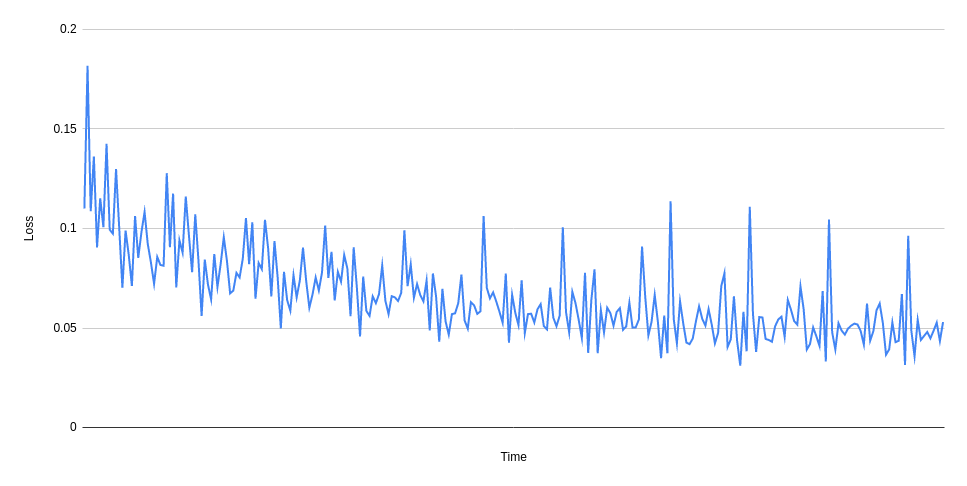
\includegraphics[width=\textwidth]{img/experiment1_results_lossOverTime.png}
		\caption{Loss over time when training with the vase images.}
	\end{subfigure}
	~ 
	\begin{subfigure}[t]{0.8\textwidth}
		\centering
		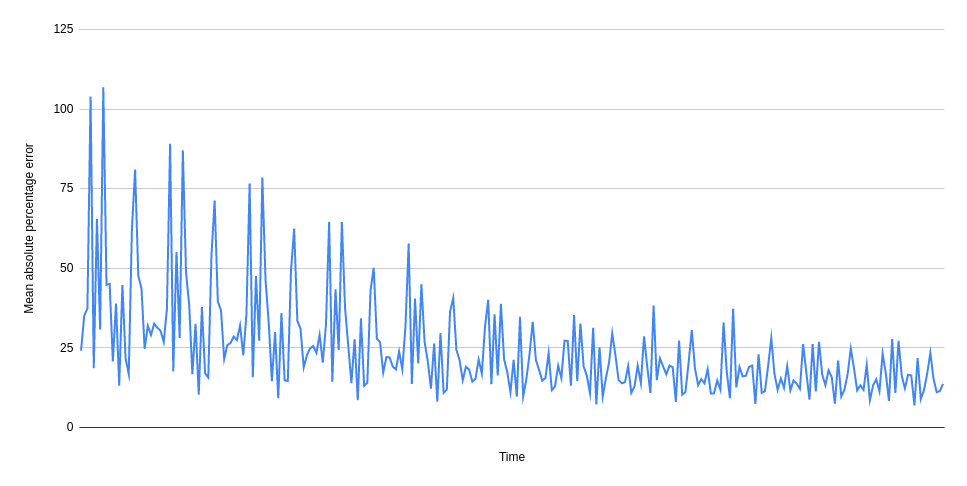
\includegraphics[width=\textwidth]{img/experiment1_results_MeanAbsolutePercentageErrorOverTime.png}
		\caption{Mean absolute percentage error over time when training with the vase images}
	\end{subfigure}
	\caption{Both, the loss and the mean absolute percentage error, decrease over time which means the predictions on vase images are getting more and more accurate.}
	\label{pic:experiment1_results_loss_and_percentageLoss}
\end{figure*}

\begin{figure*}[h!]
	\centering
	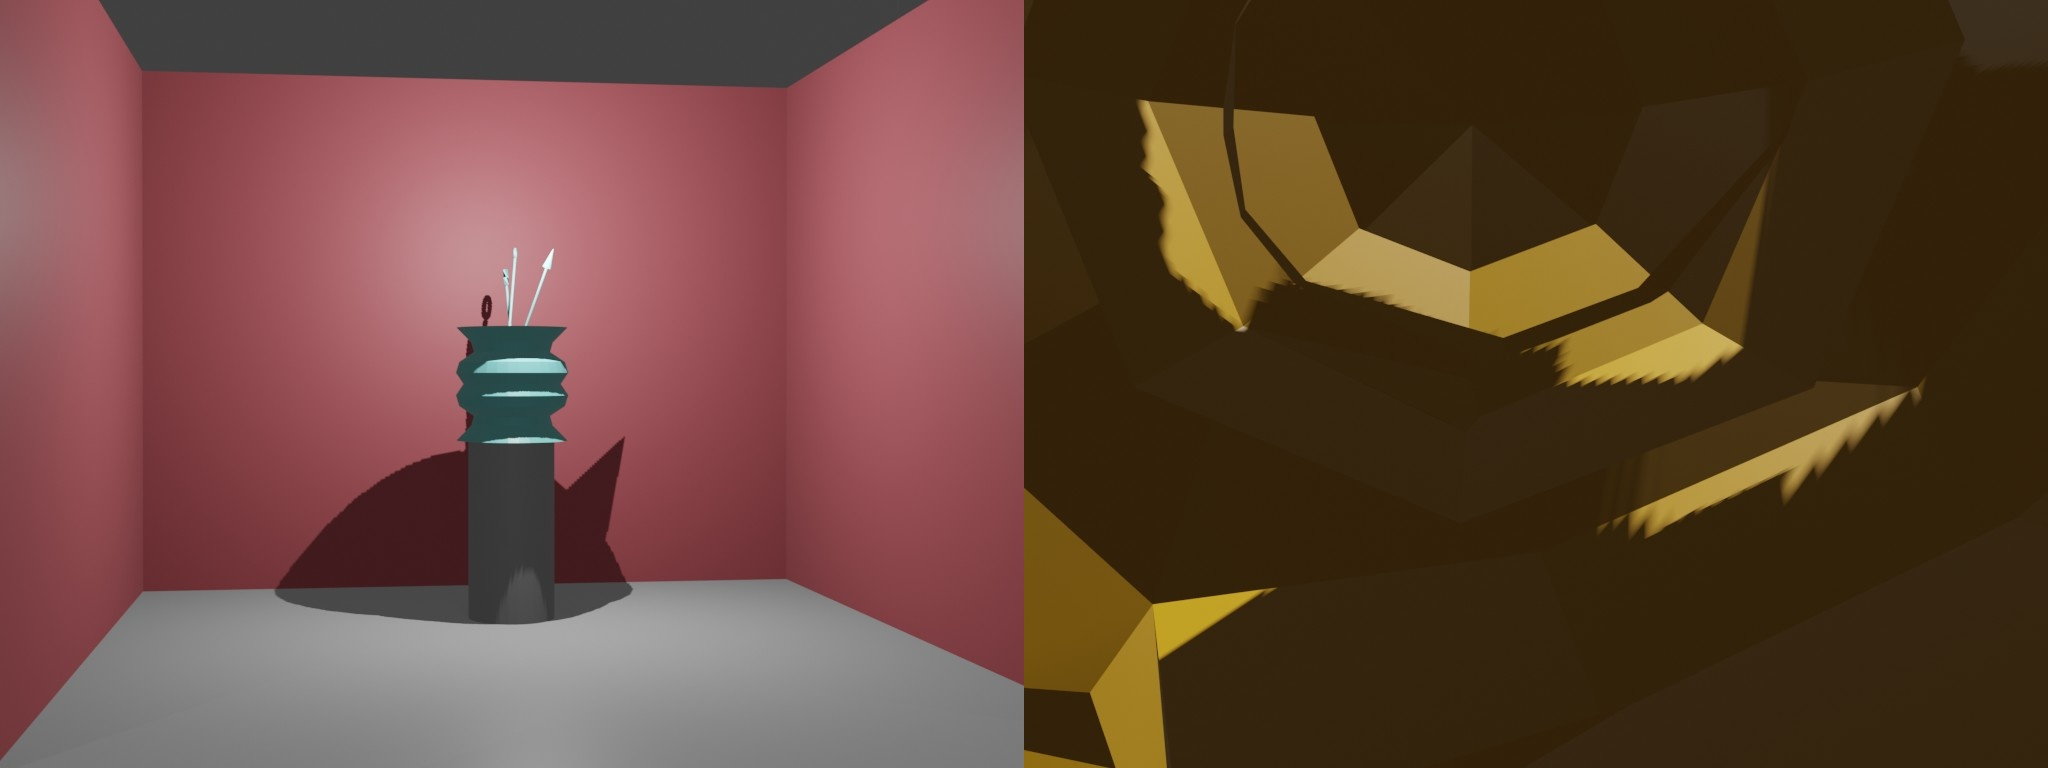
\includegraphics[width=\textwidth]{img/experiment1_results_faultyImg.jpg}
	\caption{One of the occasional faulty images. This is caused by the camera view intersecting with some objects also present in the Blender scene such as the monkey head object or the wall.}
	\label{pic:experiment1_results_faultyImage}
\end{figure*}

\section{Lessons Learned}
Looking back the most time consuming part of the Tensorflow implementation was modifications to the already existing neural network of Section~\ref{sec:implementation_neural_network}. This could have been avoided if the authors would have developed the prototype with the new hardware, where this experiment was run on, but this hardware was unavailable at the time of working on Section~\ref{sec:implementation_neural_network}, so in the future the authors will try to perform all preparations, including developing the prototype, on the same machine used in experiments.

Training a neural network with many different objects before ''showing'' it a new one could have helped improving the accuracy in this experiment. Therefore the authors recommend everyone to train on images of various objects, when the final image is not known in advance. If however, the object is known, as in the situation described in Section~\ref{sec:introduction_motivation}, training can be done specifically for the situation.

\filbreak

	\chapter{Lessons learned}

\textbf{Author: } 

\filbreak
	\chapter{Experiment 2}

\textbf{Author: } 

The second experiment is performed for the reason of testing the neural network with images of real objects. This experiment is mandatory for testing the capabilities of the neural network when it comes to real images.

\section{Preparation}
The first step of the authors was choosing a suitable object. In an effort to be time efficient once again the monkey head was chosen. This had the advantage that 3D-printing the object was easy, as all the authors had to do was exporting the existing model from Blender, and, even better, the trained weights of this object were already existing. Next the 3D model of the head was modified to include a cylindrical hole at the bottom, be able to easily mount the object. The last step was printing the object with a 3D printer. For this a Ultimaker Original and pink PLA (Polylactic acid) filament was used.

\section{Setup and Environment}
The setup consisted of a Parrot Bebop 2 and the 3D printed monkey head put on a stick to simulate the height of the head in the images produced by Blender. The authors chose a mostly white background, consisting of a table and a painted wooden board leaned on the table.

The authors were not specific about the lighting, because this experiment was to be performed as realistic as possible. For example in drone competitions the lighting often can not be influenced.

The monkey head was placed on the table facing away from the white wooden board. The drone was positioned at a distance of approximately 14cm from the object. The drone's camera was looking directly towards the object. After taking the first image the drone was moved to a second position, again about 14cm away and looking at the object. This resulted in the drone rotating slightly to the left to keep the object centred.

The images were taken with Parrot SA's FreeFlight Pro app.

\section{Sequence of Events}
The two images taken with the drone's camera from the different positions then had to be modified in order to be recognized by our neural network. The main differences between these images and the Blender generated ones were the different aspect ratio and a distortion, caused by to the way the camera operates. This can be seen in Figure~\ref{pic:experiment2_environment_comparison}. The authors wanted to make the images in (a) look like the images in (b), so modifications were necessary. The following modifications were executed with the program GIMP (GNU Image Manipulation Program), as the authors had previous experience with it:

First, the authors had to rotate the images to the left by 90 degrees, since the original images were saved in landscape. Then the authors needed to modify the aspect ratio, were cropping the image came into play. After cropping the image the final step was to get rid of the distortion. This is was relatively easy as GIMP already has a built-in distortion filter. After reversing the existing distortion the result can be seen in (c), which can then be used by our neural network to predict the distance to the drone.

Lastly the authors feed the final, undistorted images into the Neural Network, with the trained monkey head weights loaded.

\begin{figure*}[h!]
	\centering
	\begin{subfigure}[t]{\textwidth}
		\centering
		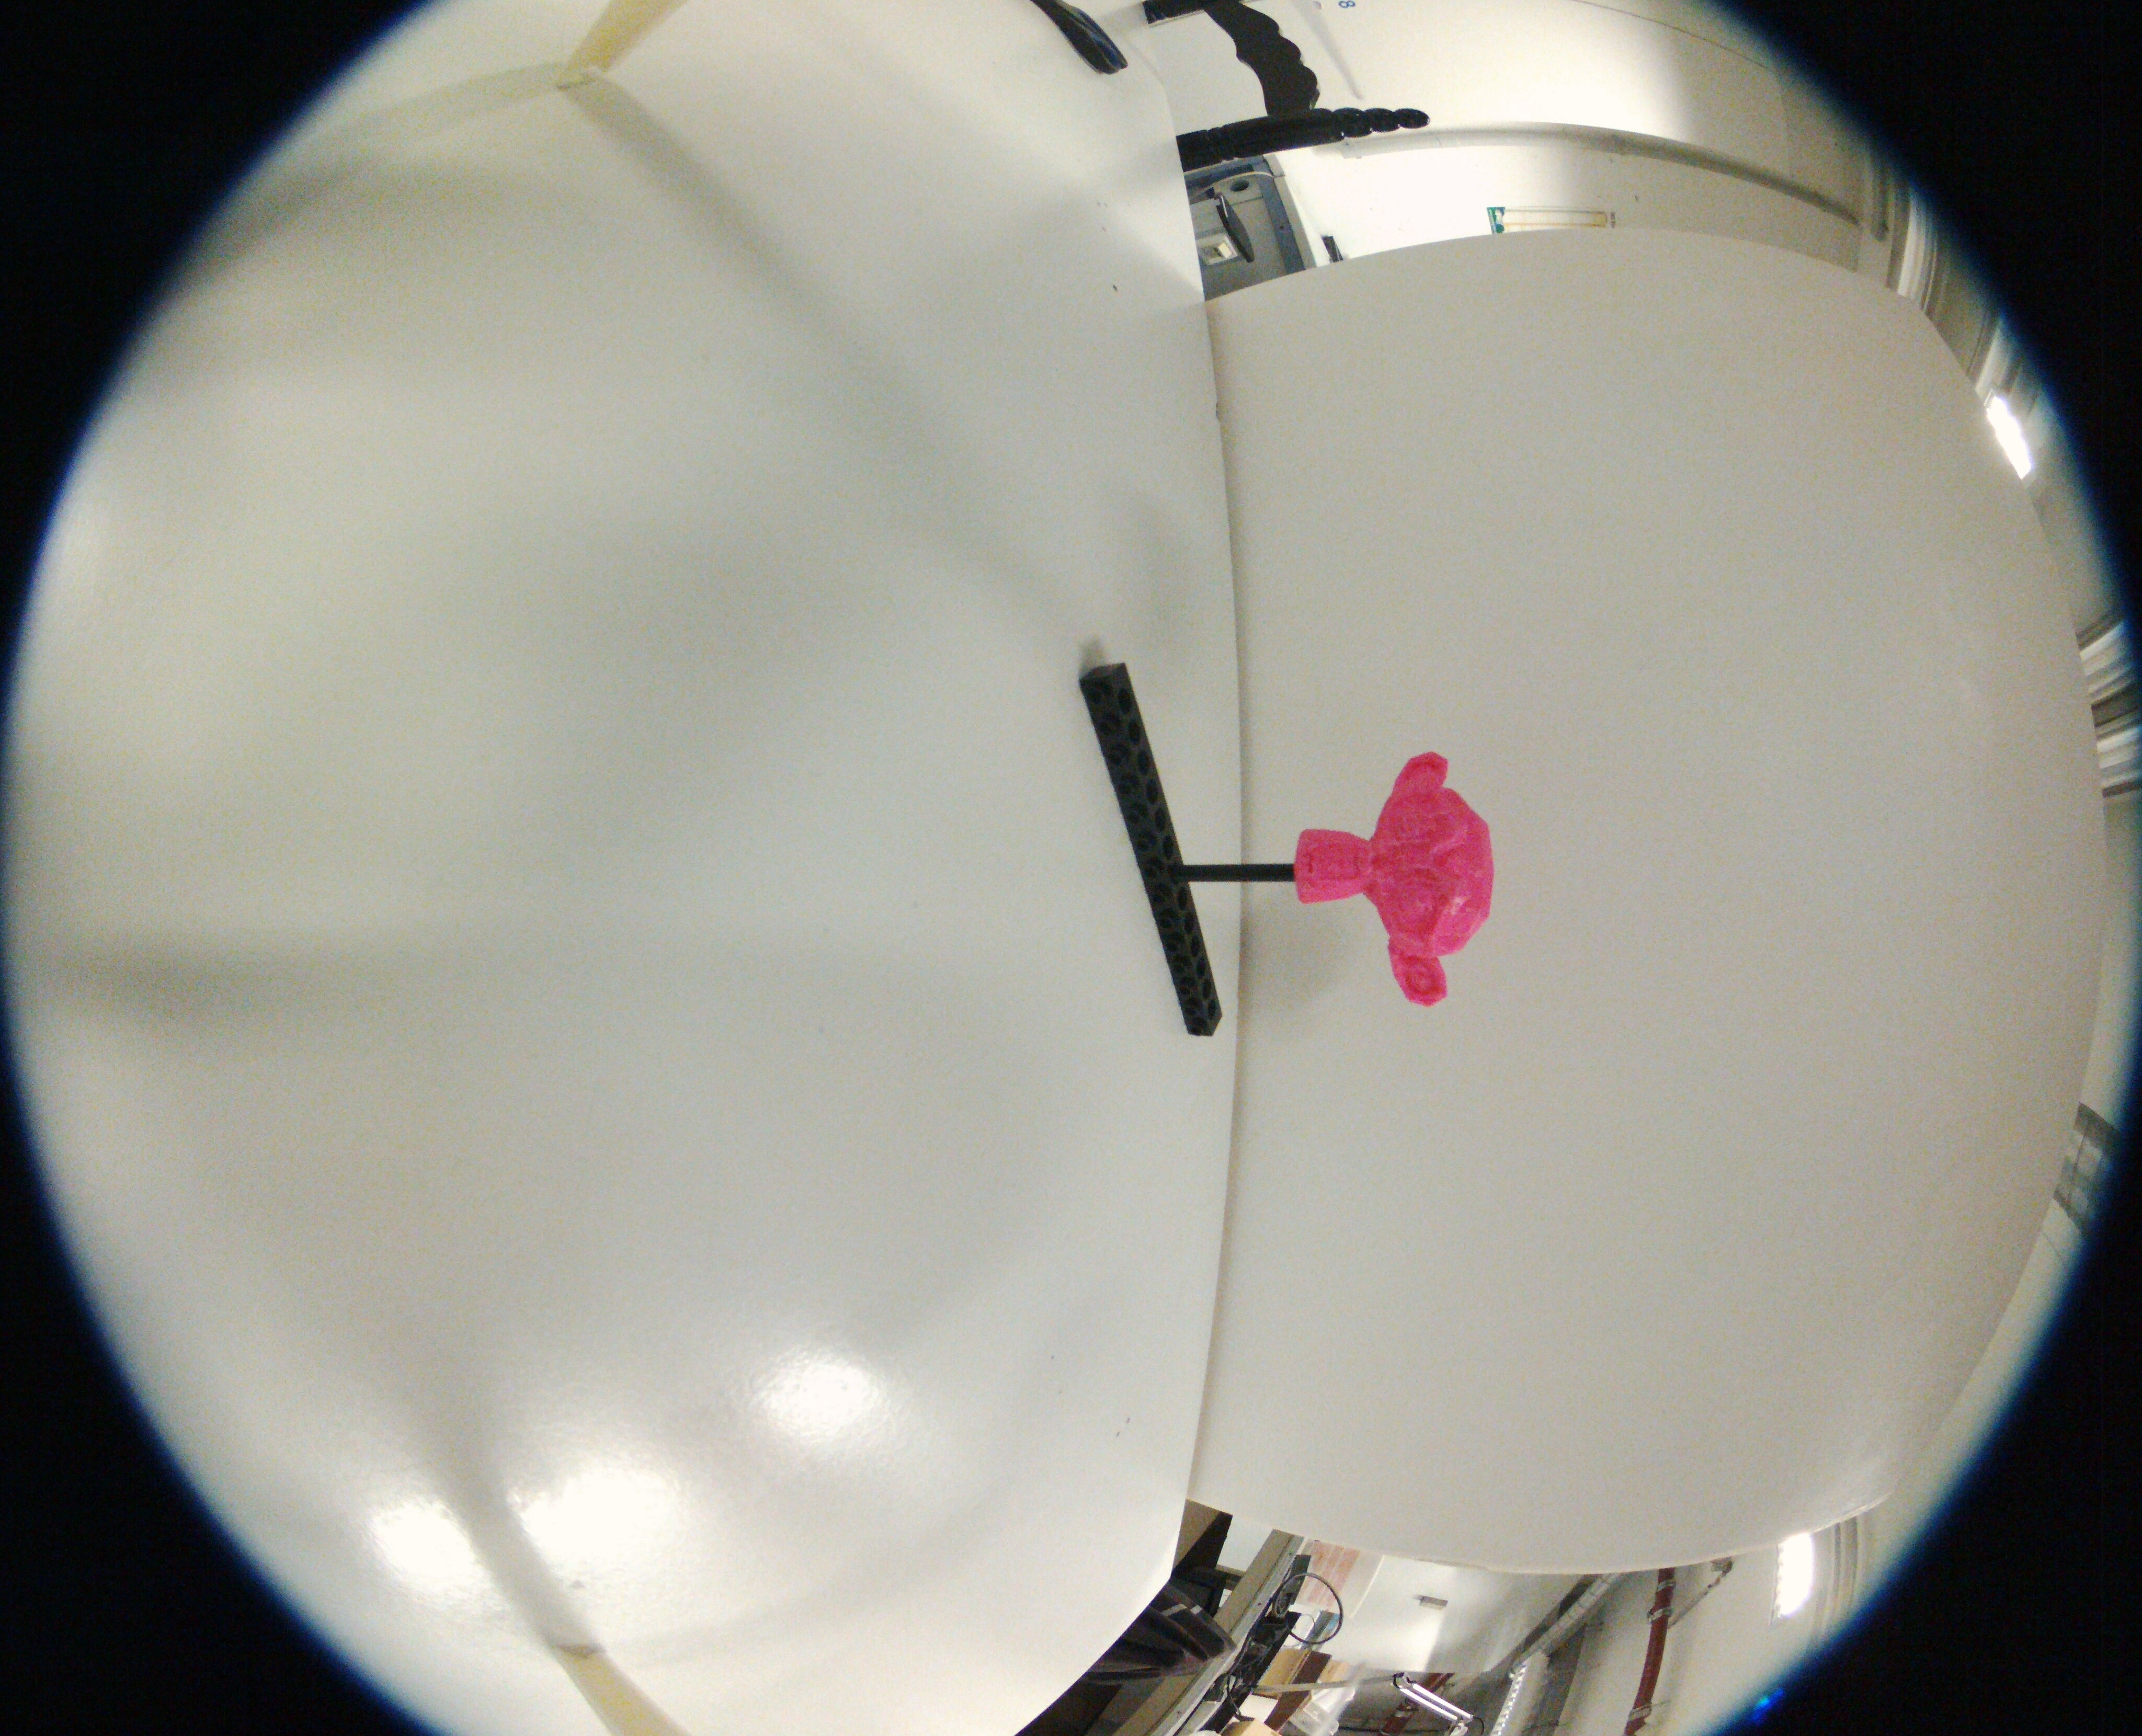
\includegraphics[width=0.48\textwidth]{img/experiment1_original_bebop_img_1.jpg}
		\hfill
		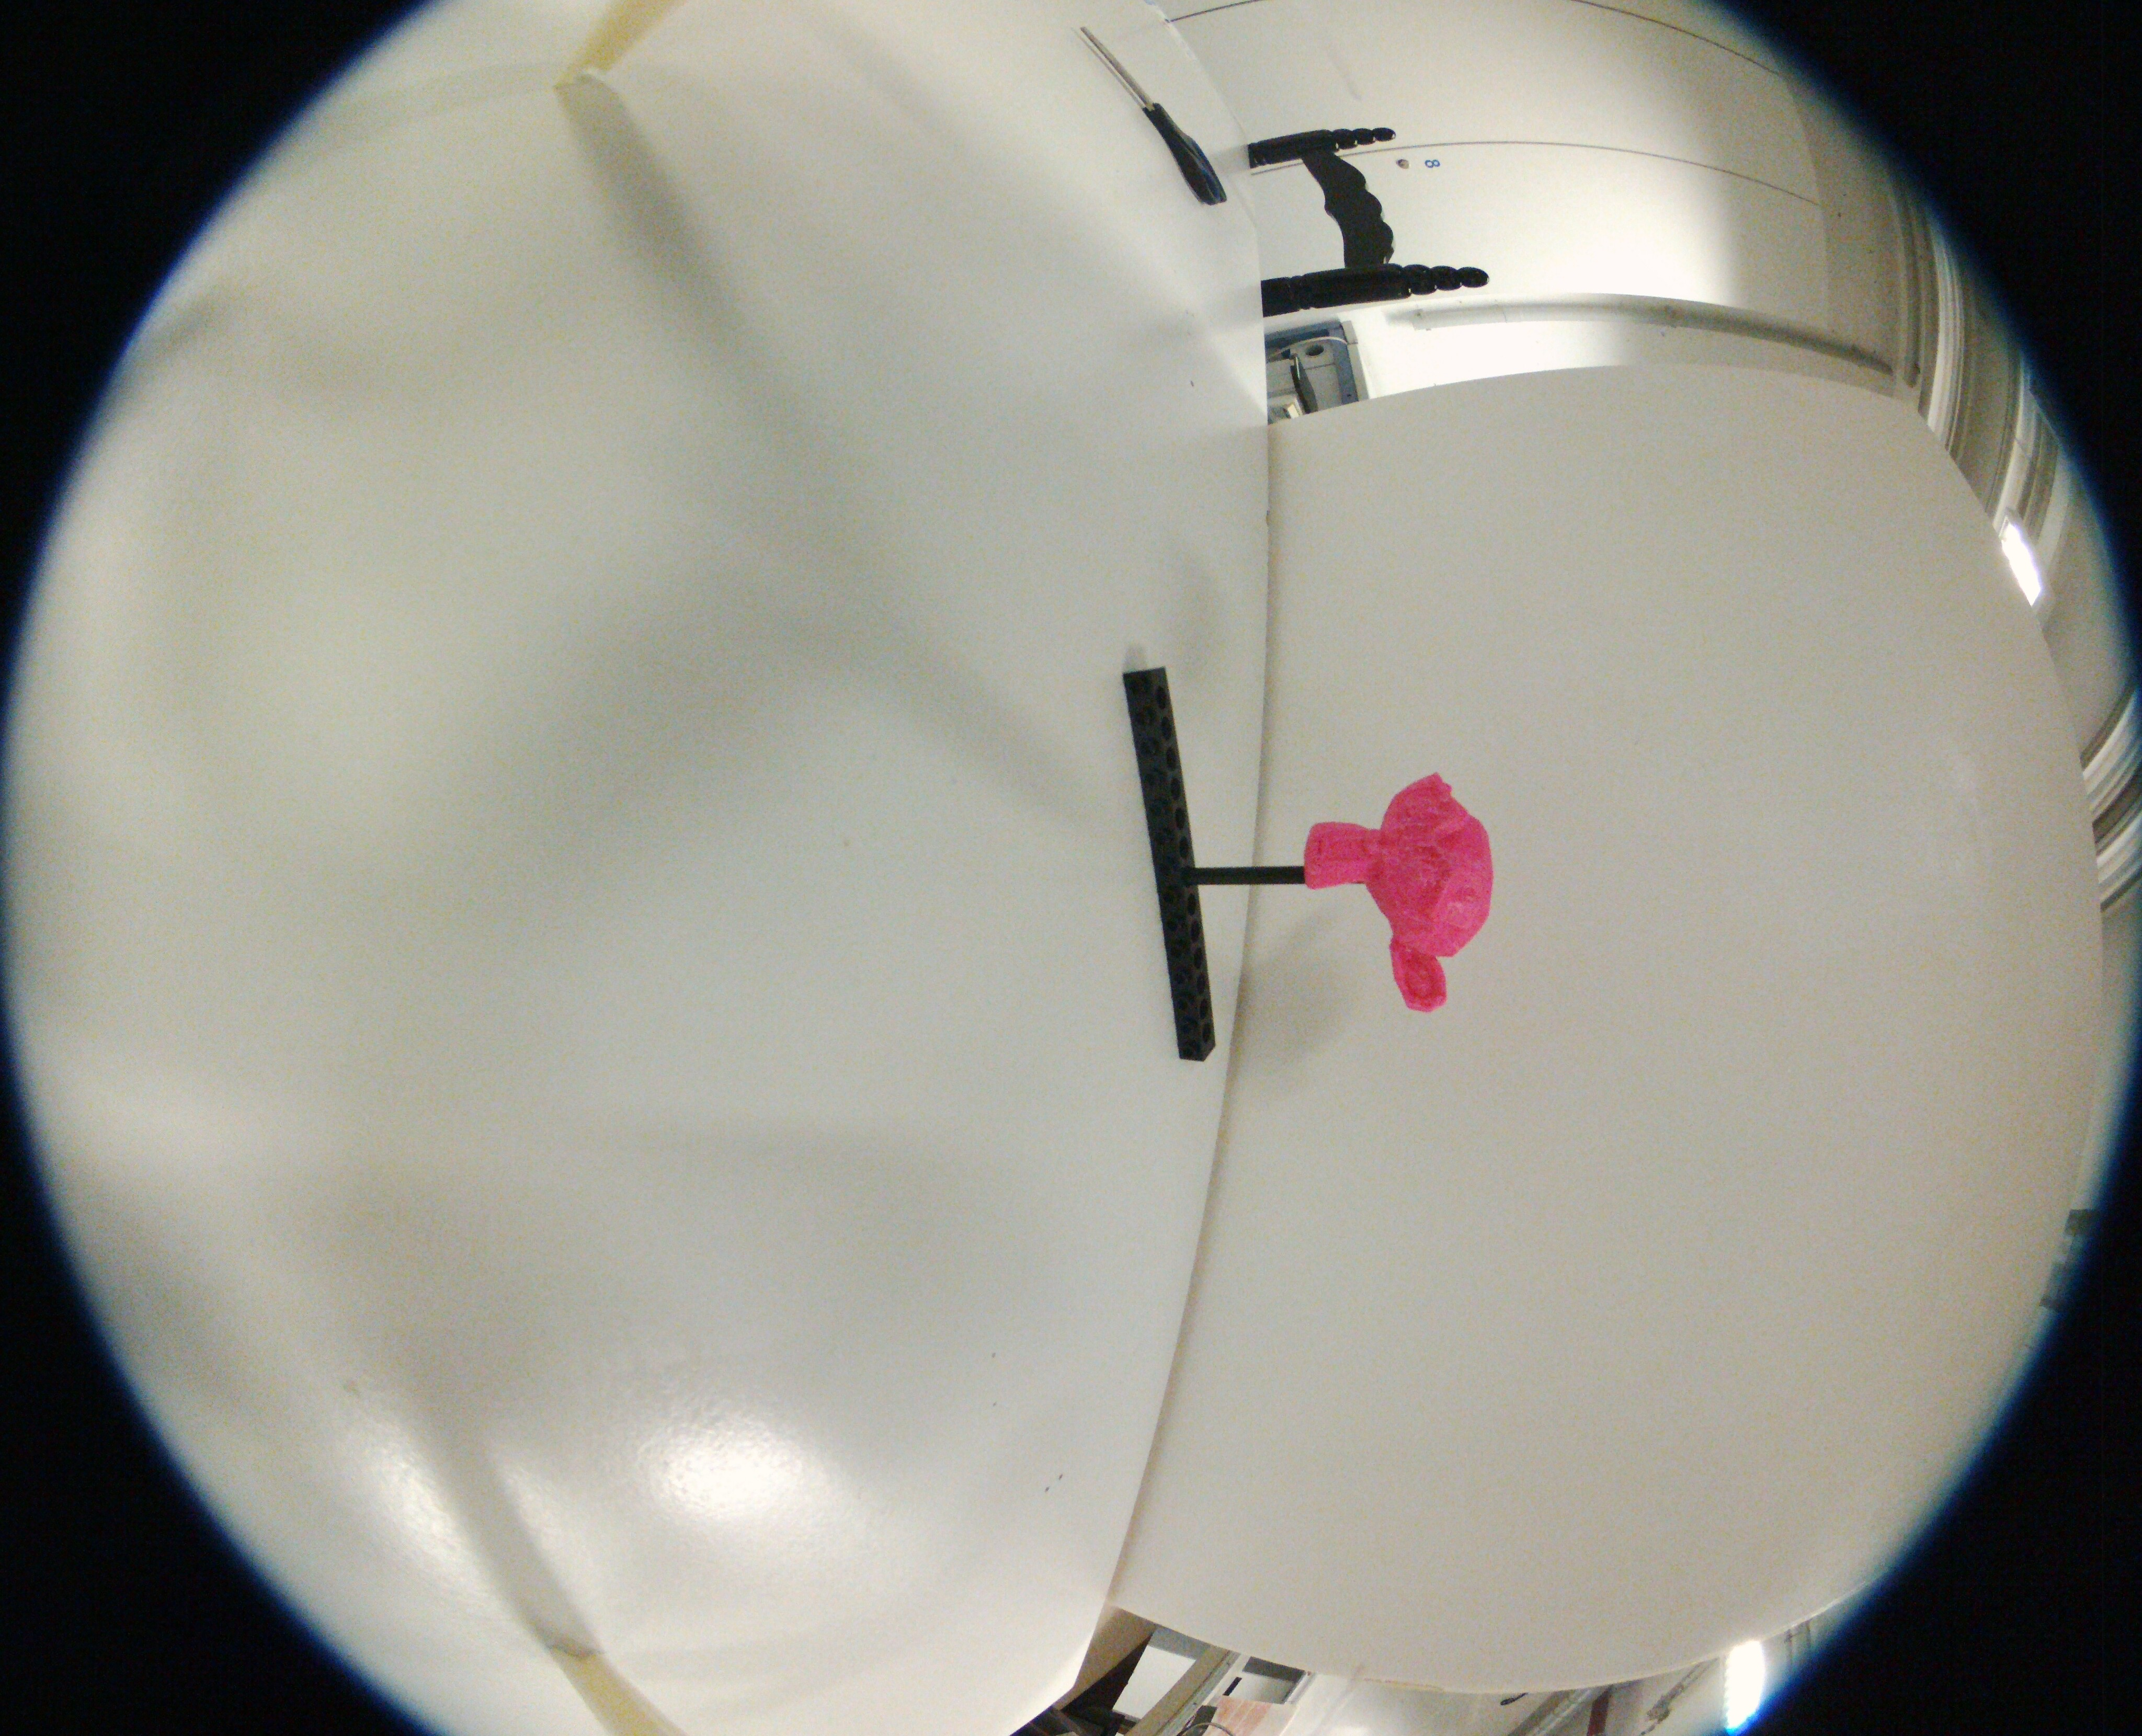
\includegraphics[width=0.48\textwidth]{img/experiment1_original_bebop_img_2.jpg}
		\caption{The original images of the 3D printed monkey head produced by the Parrot~Bebop~2.}
	\end{subfigure}
	~ 
	\begin{subfigure}[t]{\textwidth}
		\centering
		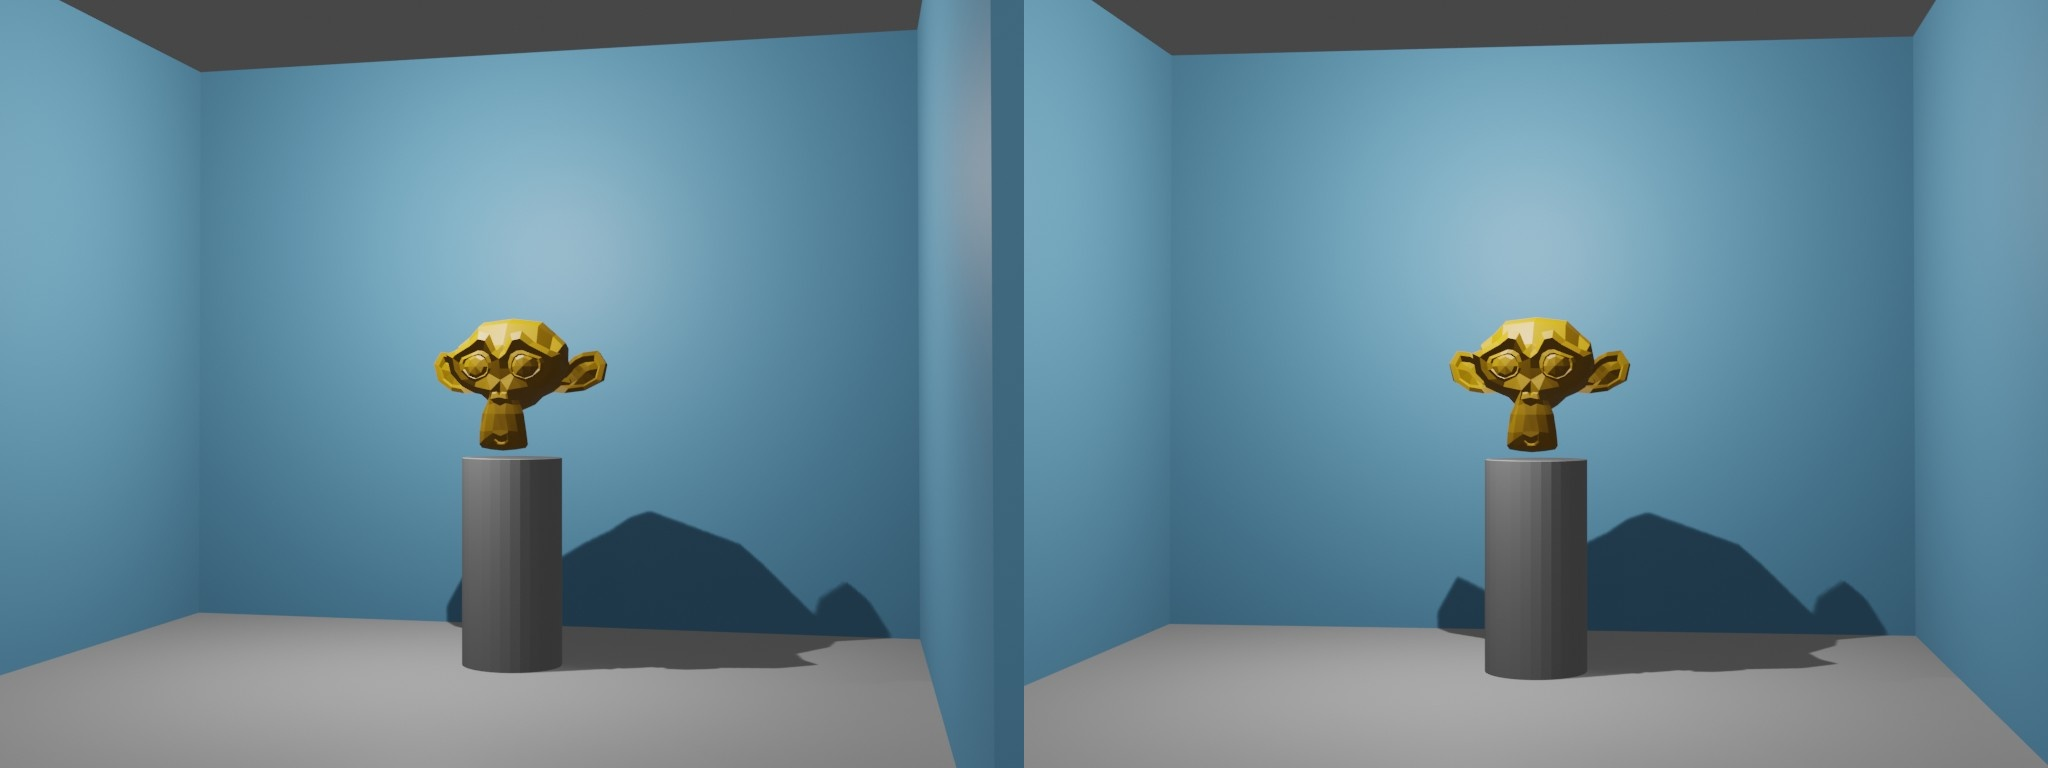
\includegraphics[width=\textwidth]{img/experiment2_environment_comparison_2.jpg}
		\caption{An example training image generated with the help of Blender.}
	\end{subfigure}
	~ 
	\begin{subfigure}[t]{\textwidth}
		\centering
		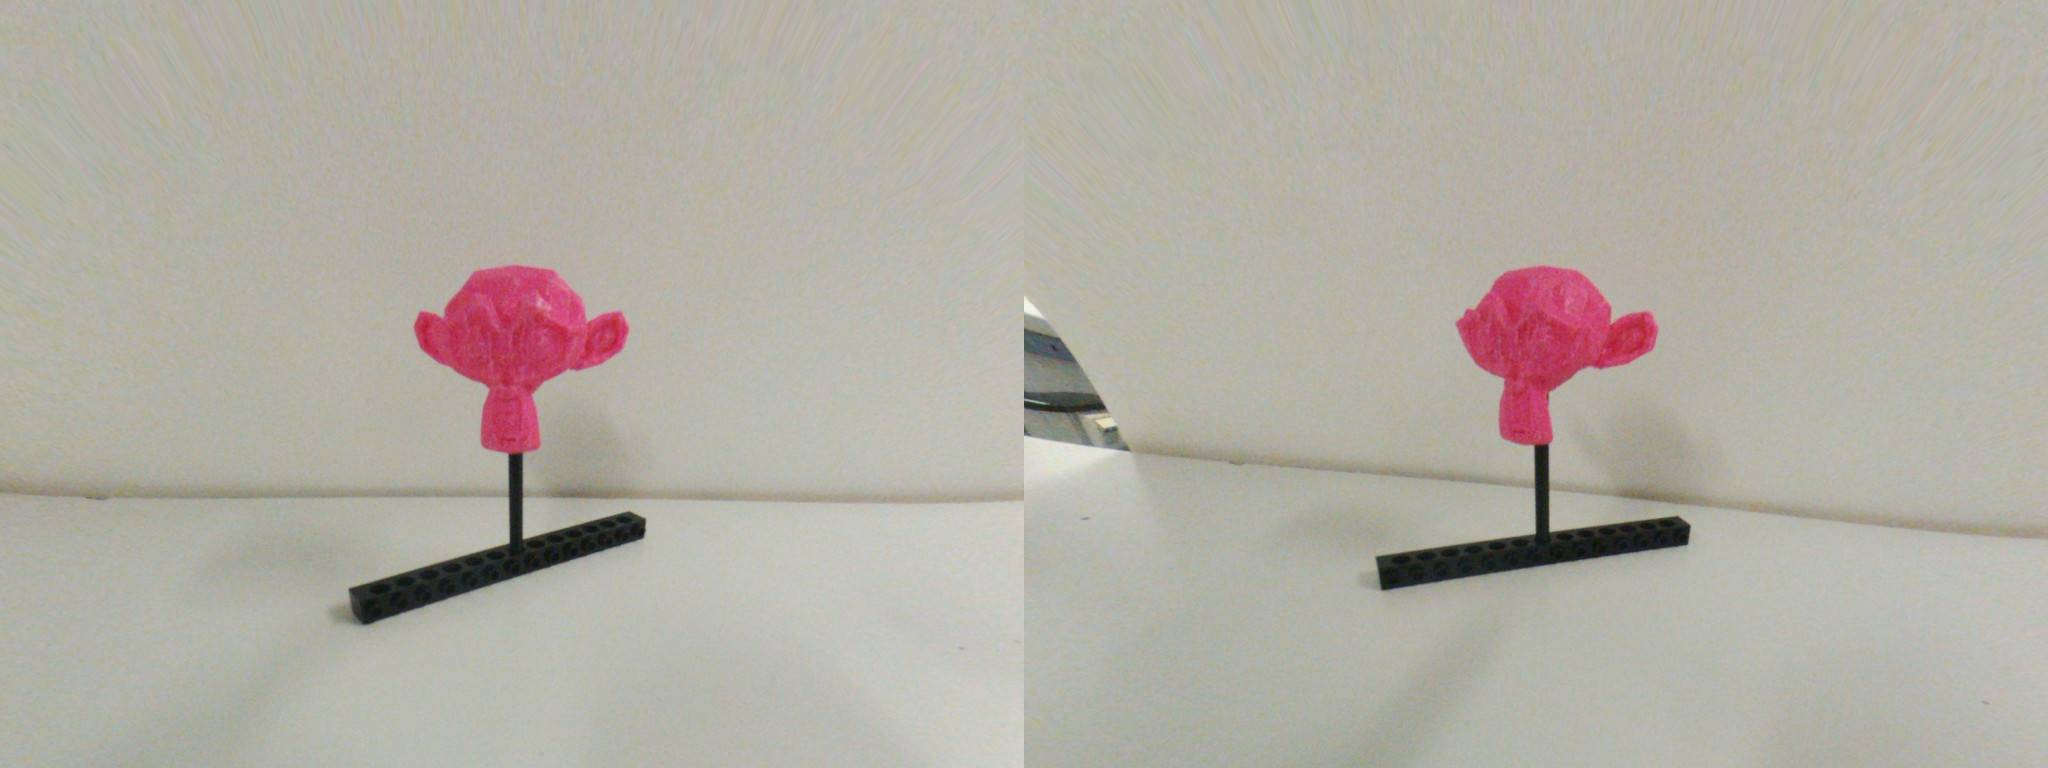
\includegraphics[width=\textwidth]{img/experiment2_environment_comparison_1.jpg}
		\caption{The two modified images of the 3D printed monkey head taken with the Parrot Bebop 2.}
	\end{subfigure}
	\caption{Image pairs of the monkey head.}
	\label{pic:experiment2_environment_comparison}
\end{figure*}

\section{Results}
Because the preparation of the images made with the Bebop Parrot 2 camera was time consuming only one pair of images was tested. The result of the prediction of this image pair was the following:

\begin{lstlisting}[]
images 0 to 1:
prediction - [3.451700 0.146270 -1.12407]    actual - [0.130000 0.030000 0.020000]
\end{lstlisting}

The fact that the prediction is off by more than one meter shows that the neural network was not able to generalise to real images. This could have multiple reasons:

\begin{itemize}
	\item the units of the scenes in Blender could not be compatible with real world units this easily,
	\item the complexity of estimating real world distances could be a more complex problem, than the limited layer neural network build by the authors can solve,
	\item the different colours of the real objects, compared to the ones in Blender, could cause confusion,
	\item the neural network could have been trained for too long (overfitting) or
	\item the missing shadow, due to the different lighting situation could have caused the problem.
\end{itemize}

It is also possible that a completely different circumstance caused the problem, but the authors could not test any hypothesis due to the limited time frame of this work.

\filbreak
	\chapter{Conclusion}

\textbf{Author: Peter Kain} 

To conclude this diploma thesis, two things became apparent: First, it does not seem possible to train a neural network with computer-generated images only and then estimate distances of real images. Second, even when evaluating distances depicted by computer-generated images, there is still some error involved. How can one fix these issues and make the neural networks more reliable for this use case?

\section{Possible Improvements}

\subsection{Input data}

In order to estimate distances of real images there currently seem to be two choices: Either taking pictures of the object by hand, or modelling a more realistic scene in Blender and take pictures the same way the authors did.

Clearly the first choice has a drawback, which is the needed effort. Taking pictures by hand is something the authors wanted to avoid from the beginning, because it is just too time consuming. One would need at least 1000 pictures of the object and would have to measure the distances to the object in the required accuracy for every picture taken.

Modelling the scene with Blender clearly seems more reasonable, because it is something one can get done after some effort. Additionally, the object and background can easily be changed to accommodate to a new situation. But some effort is still present and one will need advanced modelling skills to convincingly create a realistic scene. There also is a factor of insecurity: Before adequate testing one can not be sure if this method is working.

\subsection{Improving the Results}

Now for the second fact, the always present errors in the retrieved distance from the neural network: This is something that cannot really be fixed. Neural networks are not 100\% accurate. This can be explained by the fact that not even humans are perfect at estimating distances. The author's neural network managed to estimate distances with an accuracy of two decimal places after all of the modification described in this thesis. Humans generally can not judge distance with only their eyes and brain with the same accuracy. This is because we do not really measure distance, rather we have a feeling of how distant something is. For example when picking up an object, rather than estimating the distance and then moving our arm according to this distance, we intuitively know how we have to move our muscles to reach the desired position. Since the idea of neural networks is to train similar to the human brain, the authors do not think that small but existing errors can be eliminated. 

However, this does not mean that the always present error cannot be reduced: Both experiments use a neural network which outputs the distances to the object in x, y and z components. This can easily be simplified by just using the length of this three-dimensional vector, foregoing the information of the x, y and z coordinates and just using the length of the vector as distance to the object. This should increase the overall accuracy of the neural network, as the complexity is reduced. Similarly, using images, which have been further downscaled, also simplify the problem at hand.

The other approach to improve the accuracy is to modify the structure of the neural network and the rest of the setup to cope with more complex problems. This could be achieved by adding more layers, increasing the number of trainable parameters; using different kinds of layers in the neural network; generating more input images, to decrease overfitting or using images of various objects on different backgrounds in the training data.

There is another approach: Staying minimalistic when it comes to input data. As seen in Section~\ref{sec:implementation_neural_network} when training with only one object and the same background, the neural network's average error was 14\%, which is acceptable. In a tournament situation you may not need to train for multiple objects and backgrounds, because you may only have that one obstacle you normally would have to setup an external camera system for, and evaluate the images retrieved by the camera with a script you wrote, as was the author's case. In this case training the neural network for this one obstacle and the same background can yield results which compare to Section~\ref{sec:implementation_neural_network}, which are not that bad. An average error of 15\% lets you at least detect if something is in your way and you do not want to steer close to objects anyway.

\subsection{Switching from TensorFlow to a C++ implementation}
Since the workings of a neural network are not dependent on the programming language used, the theoretical part of this diploma thesis can be applied to self implemented neural networks as well. The C++ implementation of a neural network written by the authors will be made available to all future robotic students and can be extended to include all features necessary to perform the required estimations.

The missing features are for the most part in the development of the different layers described in Section~\ref{sec:modificationsToTheNeuralNetwork}.

Moving from a TensorFlow implementation to a C++ one can give an advantage in competitions, because you are not bound to a specific api probably everyone is using and you can expand the C++ API by adding features or optimizations specifically for the given challenge.

\newpage

\vspace{5mm}
\noindent
\textbf{Author: Ida Hönigmann}

\section{Outlook}

\subsection{Usability of this method}

Still, some problems encountered during this work are unsolved, but the authors think that the main challenge of using a neural network for this task was thoroughly explained in this thesis. Therefore the remaining work needed to get a working prototype running on a drone are limited to getting more realistic training data and wrapping the code in a few lines of instructions to the drone itself. In pseudo code these few lines look like the following:

%\newpage

\begin{lstlisting}[language=PHP]	%actually pseudo code, but php shows no syntax highlighting
takeoff drone
fly toward the general direction where the object is suspected to be
turn toward the suspected position of the object
take the first image
fly some given distance to the side
turn toward the suspected position of the object again
take the second image
merge both images into one and perform image modifications as wished
send merged image to neural network
fly toward the given output of the neural network
now the drone should be approximately at the position of the object
\end{lstlisting}

The authors conclude that future robotic students will be able to use the knowledge presented in this thesis in upcoming drone competitions, if similar challenges to the ones described in Section~\ref{sec:introduction_motivation} are posed.

\subsection{Possibilities of further development}

The authors suggest possibilities of further development of the existing code and the idea of this thesis:

\textbf{Distance estimation in mono vision cameras with the help of a neural network}

According to the visual clues used by humans to judge distance, described in Section~\ref{sec:studyOfLiterature_humanDepthPerception}, humans are able to use a multitude of monocular depth cues. Developing a working program, which estimates distance based on monocular depth cues and a neural network seems possible.

\textbf{Comparison between the work of this thesis and a stereo camera}

One way to determine if the principles described in this thesis are sufficient to get acceptable results is the comparison with a stereo camera. One could set up both methods next to each other and explore the differences in the results.

\textbf{Generating realistic Blender scenes}

One of the missing parts, to get the neural network to work in the use case described in section~\ref{sec:introduction_motivation}, is the training with realistic images. The situation of having some given object and a unknown background has to be modelled in Blender and then fed into the neural network. Afterwards one could test if this is an improvement compared to experiment 2.

\textbf{Writing a ROS (robot operating system) node from the existing code}

Lastly the authors suggest all persons wanting to use the methods described in this thesis to integrate them into a ROS node. This makes the communication to the drone easier and completely removes the problem of the image modifications needed to perform the second experiment. Capsuling the distance estimation into a node has the following advantages: debugging the code is easy, as all messages sent and received by the node can be printed, the node can easily be replaced by some different new code and the calculation can be distributed onto many different computers.

\section{Final thoughts}

All in all the authors hope to have given all readers of this thesis a deeper understanding of neural networks, their limits when it comes to processing images in search of depth information and the reasons behind computer-aided training data generation. They hope that the reader can use the obtained knowledge to get started in the development of neural networks more easily, or, if they already have previous experience with this topic, deepen their insight.

\filbreak

\end{document}
